%!TEX root = ../main.tex

\subsection{Geometric component}
\label{ss:geometric_component}

As may have become clear from the previous section, the only available information for the construction of the geometric component (and normal component) are the three vertices that define a single primitive. The vertices contain the vertex \textit{xyz} coordinates together with a unique normal per vertex i.e. the normals of each vertex is the same for every primitive using that vertex. Figure \ref{fig:method:input_primitive} contains an illustration of ``'the input primitive'' for which we will henceforward will omit the explicit reference. 

\begin{figure}
	\centering
	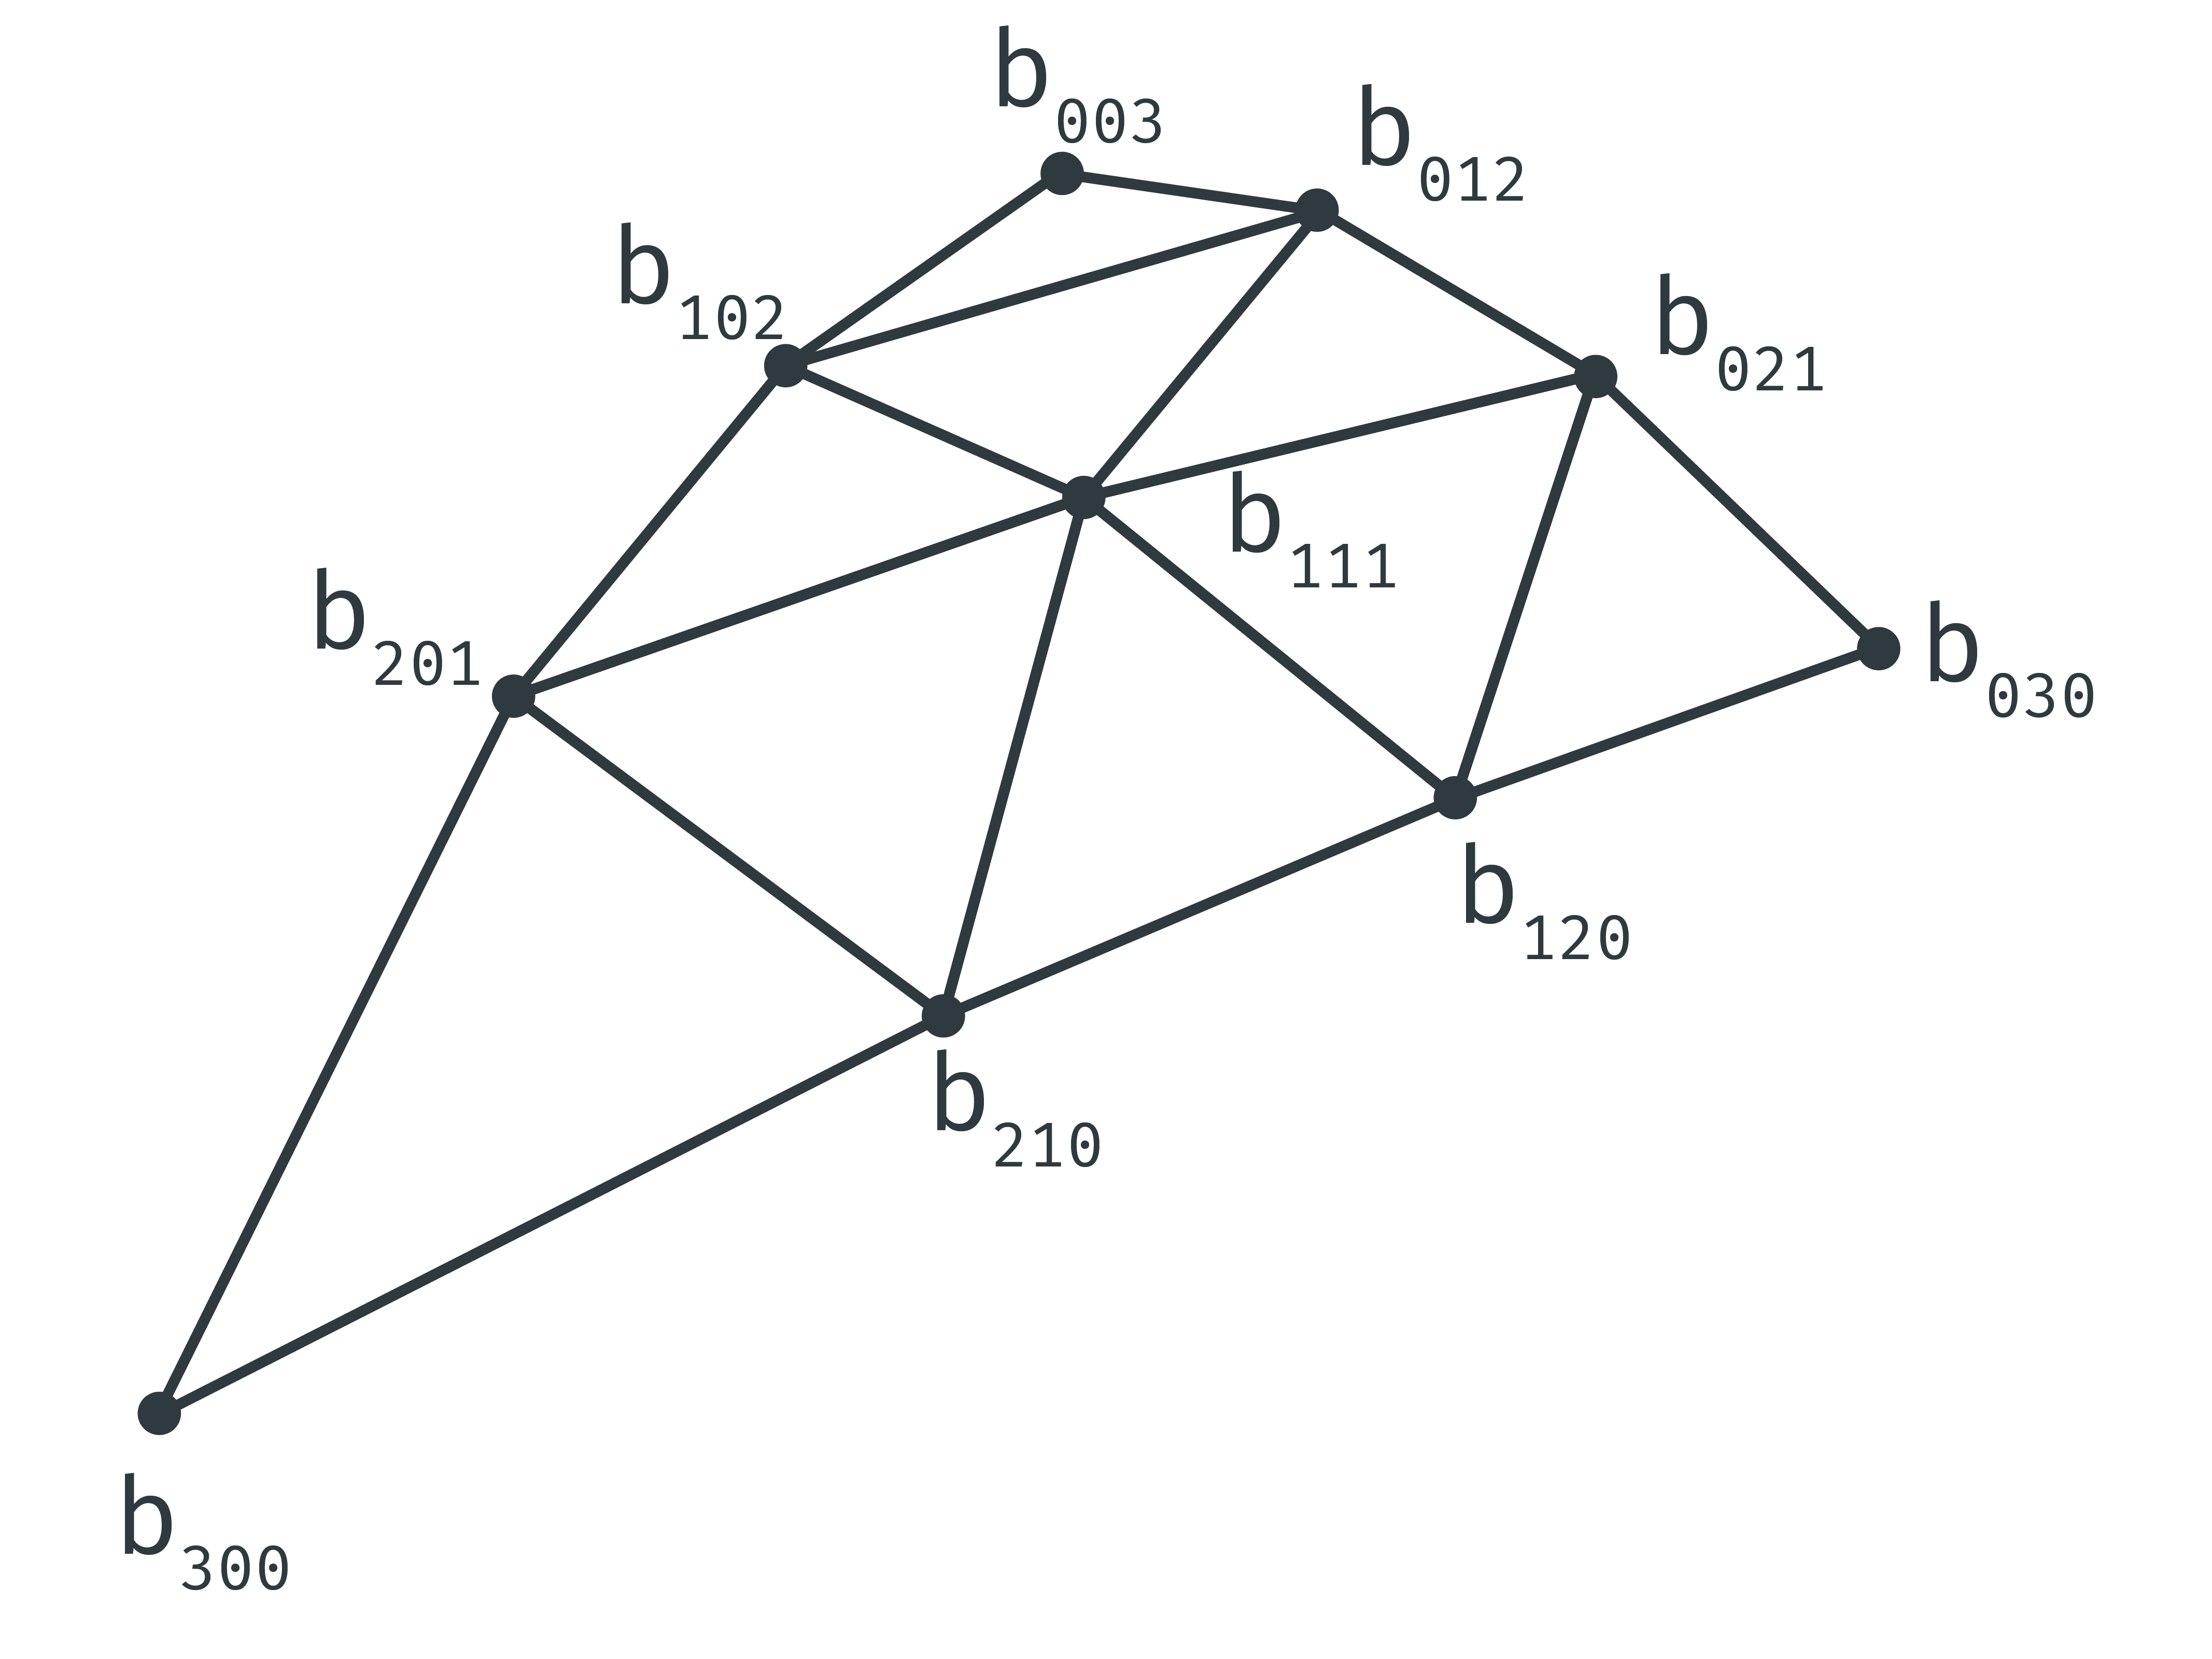
\includegraphics[width=0.45\textwidth]{./content/img/method/geometry.png}
	\caption{The geometric component: a control net of a triangular B\`ezier patch.}
	\label{fig:method:control_net}
\end{figure}

The geometric component of a PN triangle is defined by a triangular cubic B\`ezier patch, see equation \ref{eq:method:cubic_bezier_patch}. In figure \ref{fig:method:control_net} a visualization the network of the coefficients, also know as control points, is shown.

\begin{align}\label{eq:method:cubic_bezier_patch}
\begin{split}
	b: 
    a ={}& b + c + d\\
         & + e + f + g\\
      ={}& fdjsklf
\end{split}
\end{align}

Where the control points are grouped together (see figure \ref{fig:method:control_net}) as:

\begin{align}\label{eq:method:control_coefficients}
	b	
\end{align}

\todo[inline]{We express geometric compinent as a cubic patch}
\todo[inline]{Discuss parametrization of cubic patch}
\todo[inline]{Discuss the construction of the control points for the cubic patch}